\documentclass[12pt,a4paper]{article}
\setcounter{tocdepth}{4}
\usepackage[left=3cm,right=3cm,top=3cm,bottom=3cm]{geometry}
\usepackage{graphicx}
\usepackage{subcaption}
\usepackage{float}
\captionsetup{font=footnotesize}
\graphicspath{ {./images/} }

\begin{document}

    \begin{titlepage}
        \centering
        \title{COMP3419 Assignment 1\thanks{Option 1}}
        \author{Nick Zhou 460363707}
        \date{October 2018}
        \maketitle
        \centering
        
\includegraphics[width=4cm]{usyd}\\[2cm]
    \end{titlepage}

    \begin{tableofcontents}
        \tableofcontents
    \end{tableofcontents}

    \section{Introduction}

      \subsection{Preamble}

      The purpose of this report is to demonstrate the pipeline used to complete the COMP3419 Assignment (Option 1). This report consists of\
      a three main sections; introduction, implementation and conclusion. This report was created with \LaTeX{} as required by the assignment\
      specification.

      \subsection{Task}

      The task of this assignment was to program a short video involving digital video processing, compositing and 2D animation techniques.\
      The output is an animation piece based on the provided clip. The original video was of a marionette monkey with red markers on the head, hands\
      and feet. Our task involved tracking these red markets in order to determine the motion of the marionette monkey and recreate it with\
      our own character. The programming language used to complete this assignment was python3 on the windows operating system.\\

      This assignment task was broken into a set of 4 subtasks excluding this report:
      \begin{itemize}
        \item \textbf{Motion Capture}: The body of the monkey is labelled with red markers. The subtask involved the segmentation of the red markers in order to\
        track the motions of the monkey.
        \item \textbf{Replace Background and Marionette}: The blue background was to be replaced with a dynamic background. The monkey marionette was to\
        be replaced with our own character with the original motions of the old marionette being preserved.
        \item \textbf{Intelligent Objects}: Two randomly moving objects were to be added to the video and required to interact with the marionette in at least two different ways.\
        Special effects were to be triggered when the interactions between the marionette and intelligent objects occur.
        \item \textbf{Sound Track}: At least two sound tracks were to be added to the video. The sound track should be relevant to the interaction between\
        the intelligent objects and the marionette.
      \end{itemize}

    \section{Implementation}
      \subsection{Process}
        The process of implementing the assignment involved perfoming the subtasks in steps.

        \subsubsection{Capturing Motions}
        The red parts of the monkey were found by first converting the frames to HSV (Hue Saturation Value) and then applying a threshold. The\
        use of the HSV threshold to identify the red parts of the monkey proved to be far superior to using RGB. The segmentation of the red markers was\
        enhanced by performing two iterations of morphological erosion operations, followed by a single iteration dilation operation and finally\
        another iteration of erosion. An elliptical structuring element was used to perform these morphological operations.

        \begin{figure}[H]
          \centering
          \begin{subfigure}[H]{0.32\textwidth}
            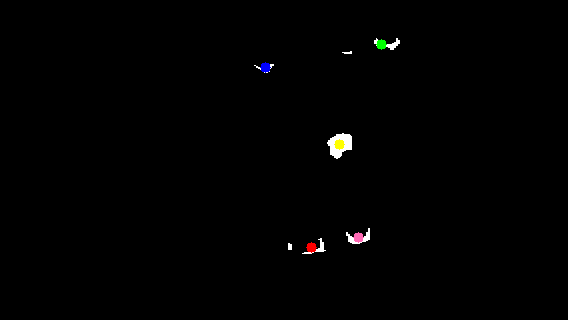
\includegraphics[width=\linewidth]{192}
            \caption{frame 1}
          \end{subfigure}
          \begin{subfigure}[H]{0.32\textwidth}
            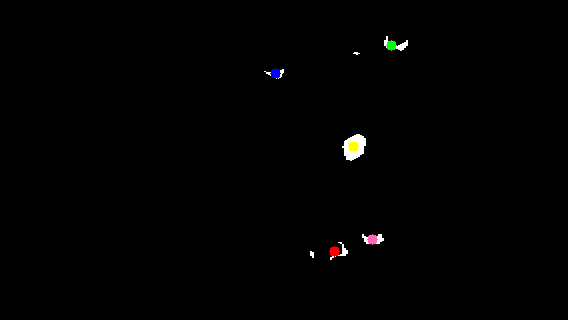
\includegraphics[width=\linewidth]{193}
            \caption{frame 2}
          \end{subfigure}
          \begin{subfigure}[H]{0.32\textwidth}
            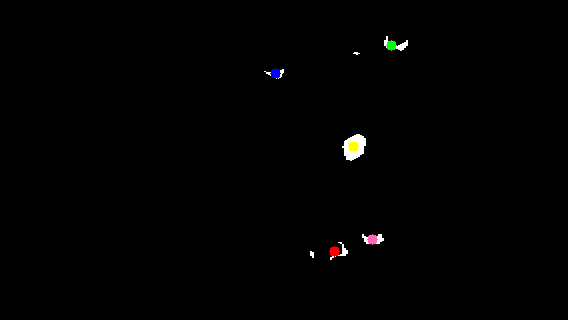
\includegraphics[width=\linewidth]{193}
            \caption{frame 3}
          \end{subfigure}
          \begin{subfigure}[H]{0.32\textwidth}
            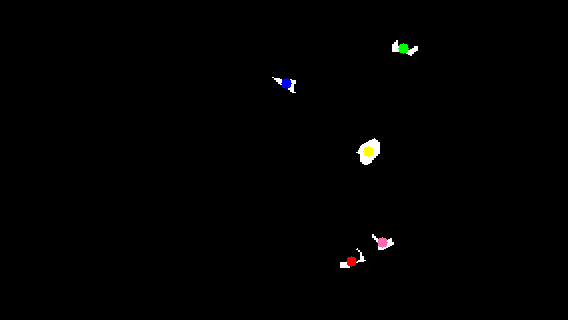
\includegraphics[width=\linewidth]{194}
            \caption{frame 4}
          \end{subfigure}
          \begin{subfigure}[H]{0.32\textwidth}
            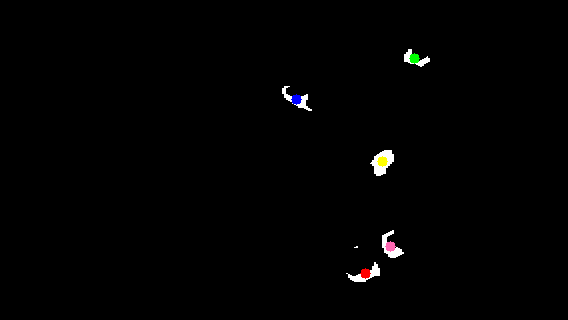
\includegraphics[width=\linewidth]{195}
            \caption{frame 5}
          \end{subfigure}
          \begin{subfigure}[H]{0.32\textwidth}
            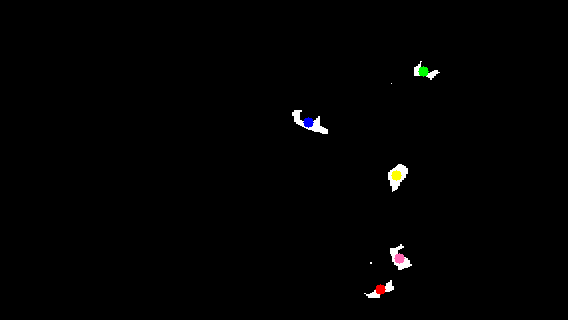
\includegraphics[width=\linewidth]{196}
            \caption{frame 6}
          \end{subfigure}
          \caption{Example of the marked centers being accurate over a series of moving frames}
        \end{figure}

        \subsubsection{Replacing Background and Marionette}
        The background is replaced by not using any part of the original video at all. Intead the only inputs in this stage from the last one are the movements of the monkey.\
        The marionette replacement is achieved by creating a Donald Trump character with each of his 5 body parts superimposed on where the monkey's red markers would have been.

        \subsubsection{Adding Intelligent Objects}
        The intelligent objects were created by loading textures from the image folder. Their movement vector is randomly chosen between\
        a sequence of -10 and 10 inclusive. Collisions between intelligent objects and marionette body parts are treated as circular objects\
        when determining their resultant velocities. When a collision between an intelligent object and marionette body part occurs, a pow image\
        is played on top of the collision area.

        \subsubsection{Adding a Sound Track}
        Whenever an intelligent object collides with the marionette, a sound track is queued to play. The sound is played using the\
        winsound library.

      \subsection{Algorithm}
      The K-Medoids algorithm was used on the red dots to distinguish them into proper clusters and identify each part of the monkey, the discernible parts being\
      the head, two arms and two legs. The initial centers of the clusters were manually set to be as close to the middle of each of the monkey\
      parts as possible.

      \subsection{Experimental Results}
      In attempting to locate the red dots on the monkey, various morphological techniques were used. Performing a closing operation resulted in \
      "clusters" that had very low dissimilarity.\\

      An opening operation yielded a result where the 5 red markers were easier to discern and had a high dissimilarity.\\

      Various other operations were performed, such as alternating between erosion and dilation operations with different number of iterations .\
      Eroding for more than 2 iterations before performing a dilation resulted in too few red pixels being retained. If the dilation was performed first,\
      the red dots joined too close to each other, which resulted in poorer cluster centers.\\

      Various structuring elements were used when experimenting with the morphological operations. A square structuring element of size 3x3\
      tended to work better than one of size 5x5. A 5x5 square structuring element would result in too much being eroded in erosion operations,\
      and too much noise with dilation operations. Though the 3x3 structuring element worked well, it was inferior to an elliptical 5x5 structuring\
      element.

    \section{Conclusion}

    The implementation of K-Medoids was highly susceptible to noise. Fast movements would often result in the deformation of the clusters.\
    The cross-over between the two legs markers did not break the clustering algorithm in matching the motions of the monkey. The\
    heavy amount of erosion performed on the image prevented the two clusters from merging into a single one.

      \subsection{Motion Capture}

      Despite the many draw backs of the implementation, all four tasks required for the assignment were certainly met successfully.\
      Most of the monkey's motions were accurately captured using the K-Medoids classifier.

      \begin{figure}[H]
        \centering
        \begin{subfigure}[H]{0.49\textwidth}
          \includegraphics[width=\linewidth]{883}
          \caption{Example of the clusters being misidentified due to noise}
        \end{subfigure}
        \begin{subfigure}[H]{0.49\textwidth}
          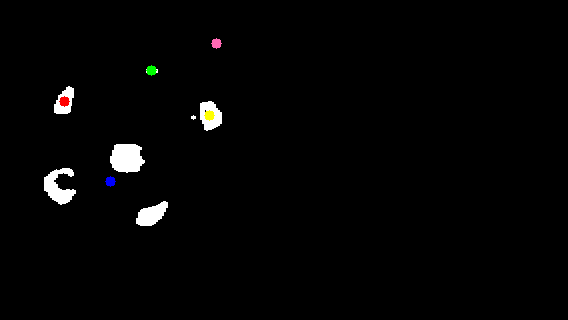
\includegraphics[width=\linewidth]{952}
          \caption{As a result of the cluster centroids being misidentified in previous frames such as the previous figure, the initial medoids result in incorrect classification of the monkey parts}
        \end{subfigure}
      \caption{When the clusters start being misclassified, future frames will also be misclassified}
      \end{figure}

      \subsection{Background and Marionette Replacement}

      The blue background and the monkey was replaced as required by the specification. The character replacement (Donald Trump) simulated the gestures of the monkey and\
      had all 5 connected components.

      \begin{figure}[H]
        \includegraphics[width=8cm]{original}
        \caption{This still shows a frame of the original video with the blue background and monkey marionette}
      \end{figure}
      \begin{figure}[H]
        \includegraphics[width=8cm]{replaced}
        \caption{This still shows a frame of the output video in which the background and marionette is replaced}
      \end{figure}

      \subsection{Intelligent Objects}

      The condition of having two intelligent objects interact with the marionette was met and their\
      motions affected when they came into contact with each other. The requirement of a special effect being trigged\
      during interactions was satisfied as demonstrated in following figure.

      \begin{figure}[H]
        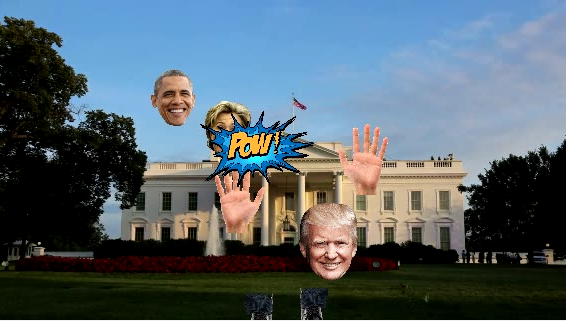
\includegraphics[width=8cm]{pow}
        \caption{A still image of a special effect being triggered when an intelligent object collides with the marionette}
      \end{figure}

      \subsection{Sound Track}

      Two soundtracks were programmed for the video. They are triggered to play when the intelligent objects collide with the marionette.\
      The sound track that is played depends on the type of intelligent object that collides with the marionette. If it is an Obama object,\
      the sound track "you're fired" is played. Alternatively, when a Hillary object collides with the marionette, the "such a nasty woman"\
      sound track is played.

      \subsection{Final Words}

      In conclusion, though the algorithms used in the implementation of the assignments tasks were not perfect,\
      they still allowed the completion of the tasks to a very high standard. Thus this report can note that this assignment\
      has been completed satisfactorily.

    \listoffigures
\end{document}
